%%%%%%%%%%%%%%%%%%%%%%%%%%%%%%%%%%%%% 
% Check out the accompanying book, Even Better Books with LaTeX the Agile Way in 2023, for a discussion of the template and step-by-step instructions. https://amzn.to/3HqwgXM https://leanpub.com/eBBwLtAW/
% The template was originally created by Clemens Lode, LODE Publishing (www.lode.de), on 1/1/2023. Feel free to use this template for your book project! 
% I would be happy if you included a short mention in your book in order to help others to create their own books, too ("Book template based on \textit{Even Better Books with LaTeX the Agile Way in 2023} by Clemens Lode").
% Contact me at mail@lode.de if you need help with the template or are interested in our editing and publishing services.
% And don't forget to follow us on Instagram! https://www.instagram.com/lodepublishing/ https://www.instagram.com/betterbookswithlatex/
%%%%%%%%%%%%%%%%%%%%%%%%%%%%%%%%%%%%%

%%%%%%%%%%%%%%%%%
% This is an excerpt from the accompanying book, Even Better Books with LaTeX the Agile Way in 2023. https://www.amazon.com/Better-Books-LaTeX-Agile-Book-ebook/dp/B0BMZJ5LF7
%%%%%%%%%%%%%%%%%


\chapter{Comparing Word and LaTeX}\label{differencebetweenwordandlatex:cha}

Everyone knows Word\index{Word@\textit{Word}}\index{Microsoft Word@\textit{Microsoft Word}|see{Word}}. However, ``knowing'' Word mostly refers to the ease of use, as it is a ``what you see is what you get'' (WYSIWYG)\index{WYSIWYG} text editor. But if I asked how to use Word to refer to another document's text block and add that as a citation in a footnote, most people would have to look on the internet to find out how that could be done. While most of Word's functionality is available through icons, you still need to know where to look when something is not a standard command\emdash{}like those used in formatting, making lists, or choosing fonts.

\begin{definition}{Word} \textit{Word} usually refers to \textit{Microsoft Word}. Generally, it is used as an umbrella term for all word processors that directly show you what you will get as an end result (as opposed to first having to process the file). This approach is intuitive, but it makes editing large projects very complicated.\end{definition}\index{Word@\textit{Word}|textbf}

In LaTeX\index{LaTeX@\textit{LaTeX}} (pronounced \ifxetex/ˈlɑːtɛx/\fi{} LAH-tekh or \ifxetex/ˈleɪtɛx/\fi{} LAY-tekh)\index{LaTeX@\textit{LaTeX}!pronunciation}, you create a text document that is then translated into an actual formatted document (your book). Formatting is done through commands you enter as text into the document. To write a LaTeX document, you never have to move your cursor, as you can enter everything by keystrokes alone.

\begin{definition}{LaTeX}\index{latex|textbf} LaTeX is a document preparation system.\end{definition}

Word and LaTeX each have particular advantages.

\textbf{If you know the commands, creating a LaTeX document will be quicker than writing a Word document.} You never have to break your concentration to access a special command. Sure, there are shortcuts in Word, but those also have to be learned.

\textbf{Because all commands are part of a LaTeX document, you can edit your text on any device with any editor you like}, while Word documents require an installed editor (well, Word) that does not show the formatting and control information.

\textbf{The upside of Word is its automated grammar check.}\index{Word@\textit{Word}!advantages} LaTeX online platforms like Overleaf\index{Overleaf@\textit{Overleaf}} provide spell checks, but no integrated grammar check. We will have to wait for future releases in that regard. 

\textbf{Word offers integrated basic graphic functionality} for symbols, while LaTeX has to rely on a rather complicated vector graphics engine.

\textbf{Editing a Word document using different versions of the software might lead to compatibility problems} and it will certainly not look the same in all versions. While there are collaborative online editors for Word, you are then on the same level as LaTeX online editors like Overleaf\index{Overleaf@\textit{Overleaf}}, and you lose the ability to work on your document while on the road without internet connectivity. Compatibility issues are especially problematic if you are co-authoring a book, working with an editor, or relying on exact page numbers. Do not forget that books can exist for quite a long time.\index{books!lifespan} Will your Word file still work in 10 or 20 years when it's time to release a new edition of your book or use parts of your book in a new book or article?

\textbf{LaTeX' more substantial post-processing of each change allows for much more complex algorithms, which provide you with better hyphenation and professional\hyp{}looking typography}\emdash{}both features come out of the box and require little to no adjusting. In LaTeX, the document is processed in the background with a delay (a few seconds up to several minutes), while Word has to provide any change in real time, which requires that editing is optimized primarily for speed. While LaTeX updates the entire document with each committed change, you need to update some elements manually in Word (for example, the table of contents and the index). 

\textbf{In LaTeX, an element of the style of the entire document can be changed with a single line of code}, while it usually takes several clicks in Word to change the style of a document. For example, in LaTeX, changing the font style of all list entries can be done centrally in one place, while in Word, you have to manually go through all of your lists to make this change.

\textbf{Changes in styles are hard to track in Word}. While Word does have a sophisticated versioning system, this applies only to the text itself. The style information (for example, the formatting of headers or footers) in Word is not part of the visible document. Hence, changes to the style are not directly visible in the document version history.\index{version history}

\begin{definition}{Versioning system} A \textit{versioning system} is a tool to track changes to a document. That means you can go back and check what has been changed and by whom.\end{definition}\index{versioning system|textbf}

\textbf{If your document contains graphics, processing Word files can become really slow, or the program might even crash.} Why? Because while you are editing, all the images have to be cached somewhere, which uses a lot of memory. When editing LaTeX documents, images in the editor are visible only by their text reference and are only later\emdash{}one by one\emdash{}automatically compiled by LaTeX into a PDF or e-book.

\textbf{LaTeX is known for its beautiful typography.}\index{typography} For example, it supports kerning\index{kerning}\index{typography!kerning} (see Figure~\ref{kerning:fig}) and ligatures\index{ligatures}\index{typography!ligatures} (see Figure~\ref{ligatures:fig}), giving a typeface its finishing touch. Improved hyphenation, proper small caps, and proper justification are other features LaTeX offers that Word cannot do as well or without additional work.

\begin{figure}[H]\centering
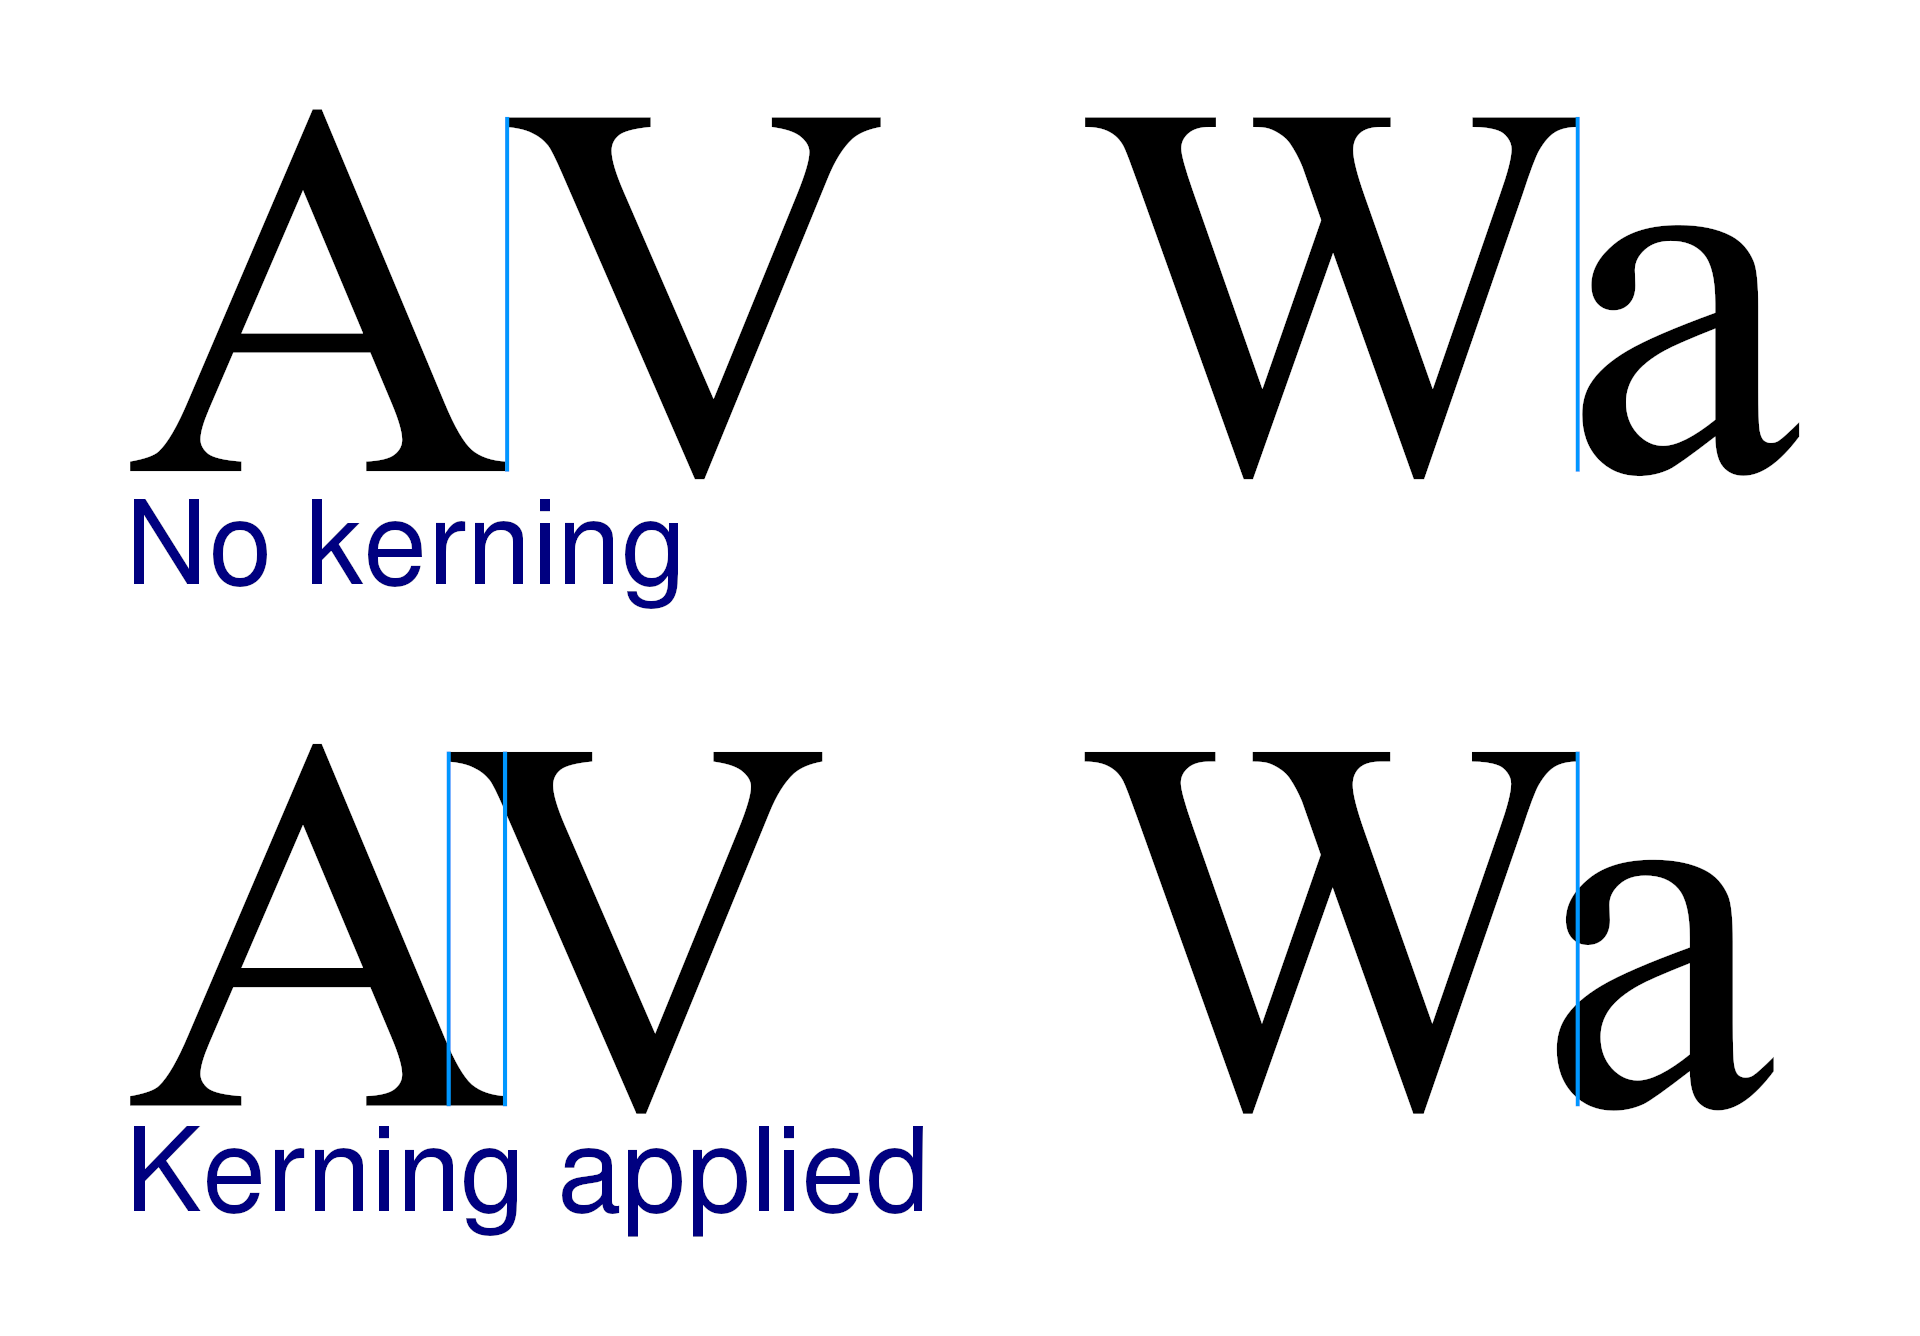
\includegraphics[width=0.25\textwidth]{images/1920px-Kerning-EN.png}
\caption{Example of kerning applied to a typeface.}
\label{kerning:fig}
\end{figure}

\begin{figure}[H]\centering
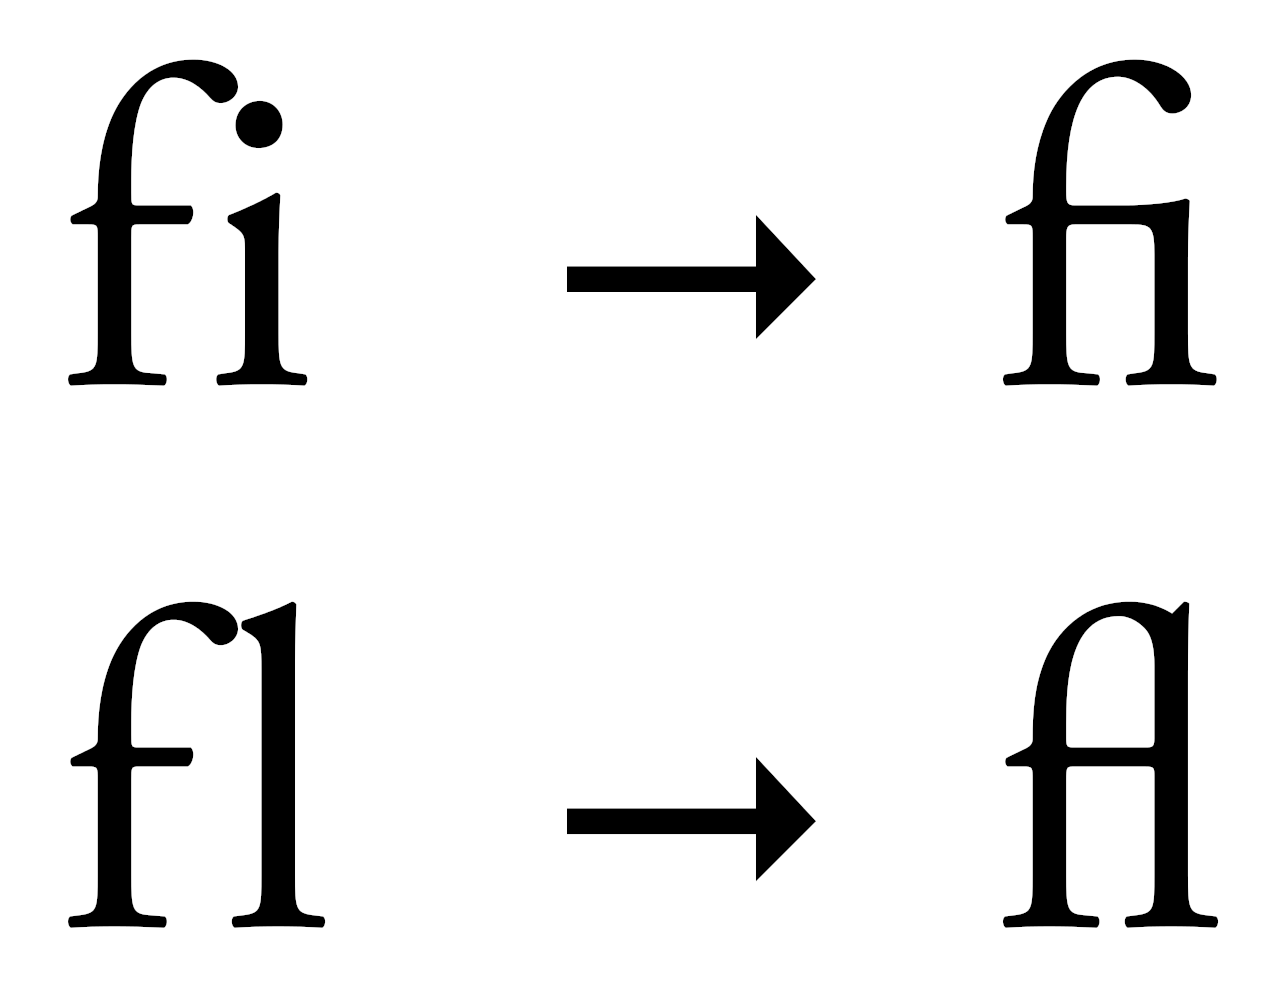
\includegraphics[width=0.25\textwidth]{images/Ligature-drawing.png}
\caption{Example of a ligature.}
\label{ligatures:fig}
\end{figure}

\textbf{While Word has several built-in tools that support multiple languages (dictionary, basic grammar check, special characters, etc.), it is not designed to handle multiple languages simultaneously.} If you want to produce, for example, a German version and an English version of your book, the best advice (using Word) would be to use two separate documents and translate and compare them paragraph by paragraph. In LaTeX, a single document can contain multiple languages.\index{multi-language project} To create a multi-language project, you can put each paragraph of the second (or third) language below the original language. This makes translation\index{translation} work more manageable and reduces work for synchronization when making revisions. This is possible by a simple switch command that uses all entries marked with either one language or with another. Check the accompanying book, (\textit{Even Better Books with LaTeX the Agile Way in 2023: Streamline Your Writing Process and Connect with Readers from Day One}, \url{https://amzn.to/3GCEGen}) for more details.

\textbf{In LaTeX, you can add functionality to switch between e-book and print output without having to manage two separate documents.} For example, my \citetitle{PFH1E} project produces four output files: the German e-book, the English e-book, the German PDF, and the English PDF. Even if your ultimate goal is to focus on the printed version of your book, merely having a more affordable e-book version will help to increase sales as it gives your readers a choice. Those who do not have a preference for reading your book in print or as an e-book might opt for the less expensive version rather than not buying your book at all.\index{price differentiation}\index{sales}

\textbf{Because LaTeX documents are compiled, you have the option to build your document not as one huge file like in Word but as a collection of many files.} As mentioned above regarding images, you can also include text files at any part of the document (as opposed to copying the whole text into one huge file). This makes it easier to divide the work and proceed section by section versus having to locate the part you are currently working on each time you open the document. It also makes rearranging sections easier: you no longer have to copy and paste pages over pages (never being sure if you have successfully copied everything and nothing was lost). Instead, you just move the \textit{reference} to a section to another place. For example, let us assume you write a book about dogs and cats and first discuss dogs, then cats. In LaTeX, you would put each discussion into a separate file and include them in your main file like this:

\begin{lstlisting}
\input{main/aboutdogs}
\input{main/aboutcats}
\end{lstlisting}

Moving your discussion about cats to the front is done by simply switching the position in the main file:

\begin{lstlisting}
\input{main/aboutcats}
\input{main/aboutdogs}
\end{lstlisting}

\textbf{If your document contains formulas, LaTeX provides an entire scientific library of functions to edit and display them directly in the document.} While you can create basic formulas in Word, you need to use a separate program to create and embed an image for any complex mathematics. Likewise, especially nonfiction books rely heavily on citations. To manage your sources in Word, you need a separate plugin or third\hyp{}party program (like \textit{Citavi}),\index{Citavi@\textit{Citavi}} while LaTeX supports the most widely used standard \textit{BibTeX}\index{BibTex@\textit{BibTex}} for free, with no plugin required.

\babelEN{\begin{definition}{Citavi} \textit{Citavi} is a plugin for Word (see \url{https://www.citavi.com}) to manage your bibliography and citations.\end{definition}}\index{Citavi@\textit{Citavi}|textbf}

\textbf{LaTeX is open source and free} (even the online editor Overleaf\index{Overleaf@\textit{Overleaf}} is free if you can do without password protection), while you have to pay license costs for Word.

\begin{figure}[H]\centering
% Diagram comparing LaTeX with Word.
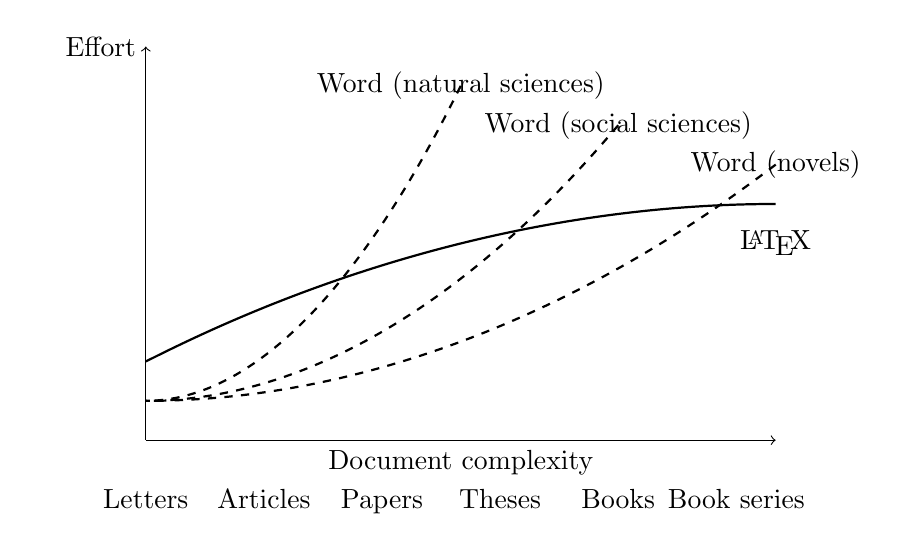
\begin{tikzpicture}

% horizontal axis
\draw[->] (0,0) -- (8,0) node[anchor=north,midway] {Document complexity};
\draw[->] (0,0) -- (0,5) node[anchor=east] {Effort};

% labels
\draw	(0,-0.5) node[anchor=north] {Letters}
		(1.5,-0.5) node[anchor=north] {Articles}
		(3,-0.5) node[anchor=north] {Papers}
		(4.5,-0.5) node[anchor=north] {Theses}
		(6,-0.5) node[anchor=north] {Books}
		(7.5,-0.5) node[anchor=north] {Book series};

\draw (8,3.5) node {Word (novels)};
\draw (6,4) node {Word (social sciences)};
\draw (4,4.5) node {Word (natural sciences)};
\draw (8,2.5) node {\LaTeX{}};

% Psis
\draw[thick,dashed] (8,3.5) parabola[bend at end] (0,0.5);
\draw[thick,dashed] (6,4) parabola[bend at end] (0,0.5);
\draw[thick,dashed] (4,4.5) parabola[bend at end] (0,0.5);
\draw[thick] (0,1) parabola[bend at end] (8,3);
\useasboundingbox (-1.5,-0.2);
\end{tikzpicture}
\caption{Comparison of Word and LaTeX depending on the complexity of the task: for natural sciences, anything more complex than articles takes more effort in Word; for social sciences, anything more complex than papers takes more effort in Word; for novels, book series take more effort in Word than in LaTeX.}
\label{latex-effort-writing-complexity:fig}
\end{figure}

Ultimately, it depends on your needs. If you want to write a complex document like a book, the advantages of LaTeX outweigh those of Word. If you want to quickly write a few pages, Word is superior. For longer and more complex books, LaTeX takes less effort (see Figure~\ref{latex-effort-writing-complexity:fig}). In this book, I will help you to get your book done and published with LaTeX using the free template provided with the book.\index{LaTeX@\textit{LaTeX}!free book template}

\begin{figure}[H]\centering
\resizebox{\textwidth}{!}{\begin{tabular}{p{.2\textwidth}|p{.4\textwidth}|p{.4\textwidth}}
\hline
&\textbf{Word}&\textbf{LaTeX}\\\hline
Editor&``what you see is what you get''&source file is compiled\\\hline
Compatibility&dependent on editor&independent of editor\\\hline
Graphics&simple inbuilt editor, mouse-based&powerful but complex editor, text-based\\\hline
Typography&optimized for speed&optimized for quality\\\hline
Style&inbuilt style&separate style document\\\hline
Multi-platform&only via export&possible with scripting\\\hline
Refresh&some elements need manual refresh&everything is refreshed with each compile\\\hline
Formulas&basic support needs external tools&complete support\\\hline

\end{tabular}}
\caption{Comparison of Word and LaTeX}
\label{comparisonwordlatex:fig}
\end{figure}

\textbf{Summary:} Word is great for quickly writing a few pages, while LaTeX is better for more complex documents such as books. LaTeX provides better typography, graphics, compatibility, and multi-platform support than Word, but it requires learning the commands and therefore using LaTeX might take longer to create a document.